\chapter{Виджеты кнопок}
{\bfseries gtkmm} предоставляет четыре основных типа кнопок: 


{\bfseries Обычные кнопки (Push-Buttons) }
Представлены классом Gtk::Button, стандартные кнопки, обычно снабженные надписью или картинкой. Нажатие приводит к выполнению действия. Подробнее в разделе "Кнопка (Button)". 

{\bfseries Кнопки-переключатели (Toggle buttons) }

Представлены классом Gtk::ToggleButton. В отличие от обычной кнопки, кнопка-переключатель остается в нажатом состоянии до того момента, пока вы снова не нажмете на нее. Данные кнопки могут быть полезны для реализации переключателя состояний включено/выключено. Подробнее в разделе "Кнопка-переключатель (ToggleButton)". 

{\bfseries Флажки (Checkboxes)}

Представлены классом Gtk::CheckButton. Ведут себя точно так же, как и кнопки-переключатели, но отображают свое состояние с помощью небольших квадратов, снабженных расположенными сбоку строками описания. Их следует использовать в большинстве случаев, когда требуется осуществить переключение состояния включено/выключено. Подробнее в разделе "Флажок (CheckBox)". 

{\bfseries Радио-кнопки (Radio Buttons)}

Представлены классом Gtk::RadioButton. Названные ввиду схожести с переключателями станций в старых автомагнитолах, эти кнопки используются в составе групп для выбора взаимоисключающих параметров. Нажатие на одну из кнопок приводит к отключению всех остальных кнопок группы. Они аналогичны флажкам (небольшим виджетам со строкой описания сбоку), но выглядят по-другому. Подробнее в разделе "Радио-кнопка (RadioButton)". 

Следует учесть, что из-за использования системы тем GTK+ внешний вид описанных виджетов может быть различным. В случае флажков и радио-кнопок различия могут быть значительными. 

\section{Кнопка (Button)}
\subsection{Конструкторы}
 Существует два способа создания кнопки. Вы можете указать строку для надписи на кнопке при использовании конструктора класса Gtk::Button или установить эту строку позднее с помощью метода set\_label().
Для активации акселератора кнопки, предназначенного для навигации с помощью клавиатуры, следует поместить символ подчеркивания перед одним из символов строки для надписи на кнопке и использовать логическое значение true в качестве значения дополнительного аргумента mnemonic, регламентирующего использование мнемоник. Например:

Gtk::Button* pButton = new Gtk::Button("\_Something", true);

Всегда, когда это возможно, вам следует использовать стандартные кнопки (Stock Items) для достижения единообразия внешнего вида вашего приложения со сторонними приложениями, а также для улучшения внешнего вида ваших приложений посредством использования иконок. Например:

Gtk::Button* pButton = new Gtk::Button(Gtk::Stock::OK);

Для данной кнопки будет использоваться стандартный текст надписи на всех языках, а так же стандартные клавиатурные акселераторы и стандартная иконка.

Виджет, представленный классом Gtk::Button также является контейнерным, поэтому вы можете помещать в него любой другой виджет, такой, как представленный классом Gtk::Image виджет для вывода картинки. 
\subsection{Пример}
Данный пример позволяет создать кнопку с иконкой и надписью. 
\begin{figure}[h]
	\center{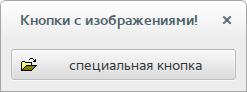
\includegraphics[width=1\linewidth]{51}}
	\caption{Пример использования кнопок.}
	\label{ris5:image}
\end{figure}
Файл buttons.h (Для использования совместно с gtkmm 3, а не с gtkmm 2) 
\begin{lstlisting}[language=C++]
#ifndef GTKMM_EXAMPLE_BUTTONS_H
#define GTKMM_EXAMPLE_BUTTONS_H

#include <gtkmm/window.h>
#include <gtkmm/button.h>

class Buttons : public Gtk::Window
{
public:
	Buttons();
	virtual ~Buttons();

protected:
	void on_button_clicked();
	Gtk::Button m_button;
};

#endif

\end{lstlisting}
Файл buttons.cpp (Для использования совместно с gtkmm 3, а не с gtkmm 2) 
\begin{lstlisting}[language=C++]
#include "buttons.h"
#include <iostream>

Buttons::Buttons()
{
	m_button.add_pixlabel("info.xpm", "special button");
	set_title("Button with picture!");
	set_border_width(10);
	
	m_button.signal_clicked().connect( sigc::mem_fun(*this,
		&Buttons::on_button_clicked) );

	add(m_button);

	show_all_children();
}

Buttons::~Buttons()
{
}

void Buttons::on_button_clicked()
{
	std::cout << "Button is pressed" << std::endl;
}
\end{lstlisting}

\subsection{Сигналы}
Виджет, представленный классом Gtk::Button, генерирует приведенные ниже сигналы, но в большинстве случаев вам придется обрабатывать исключительно сигнал "clicked":

{\bfseries pressed}
Генерируется в момент нажатия кнопки. 

{\bfseries released}
Генерируется в момент отпускания кнопки. 

{\bfseries clicked}
Генерируется после того, как кнопка нажата и отпущена. 

{\bfseries enter}
Генерируется в момент, когда указатель мыши перемещается над окном кнопки. 

{\bfseries leave}
Генерируется в момент, когда указатель мыши покидает окно кнопки. 

\section{Кнопка-переключатель (ToggleButton)}
 Кнопки-переключатели (представленные классом Gtk::ToggleButton) похожи на обычные кнопки (представленные классом Gtk::Button), но после нажатия они остаются активированными или нажатыми до того момента, пока снова не будут нажаты.

Для получения состояния кнопки-переключателя вы можете использовать метод get\_active(). Он возвращает логическое значение true в том случае, если кнопка "утоплена". Вы также можете установить состояние кнопки-переключателя с помощью метода set\_active(). Следует учесть, что в том случае, если вы сделаете это и состояние кнопки изменится, будет сгенерирован сигнал "clicked". Эти методы используются чаще всего.

Вы можете использовать метод toggled() для изменения состояния кнопки вместо четкой установки того, должна ли кнопка находиться в обычном состоянии или быть утоплена: этот метод переключает состояние кнопки и приводит к генерации сигнала "toggled".

Класс Gtk::ToggleButton важен, так как является базовым классом для классов Gtk::CheckButton и Gtk::RadioButton. 

\section{Флажок (CheckButton)}
Класс Gtk::CheckButton наследуется от класса Gtk::ToggleButton. Единственным реальным различием между представленными этими классами виджетами является внешний вид виджета, представленного классом Gtk::CheckButton. Вы можете проверять состояние виджета, устанавливать, а также изменять его используя те же методы, которые реализованы в рамках класса Gtk::ToggleButton. 

\subsection{Пример}
\begin{figure}[h]
	\center{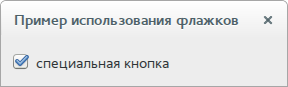
\includegraphics[width=1\linewidth]{52}}
	\caption{Флажок (CheckButton)}
	\label{ris:image1}
\end{figure}

Файл examplewindow.h (Для использования совместно с gtkmm 3, а не с gtkmm 2)
\begin{lstlisting}[language=C++]
#ifndef GTKMM_EXAMPLE_BUTTONS_H
#define GTKMM_EXAMPLE_BUTTONS_H

#include <gtkmm/window.h>
#include <gtkmm/checkbutton.h>

class ExampleWindow : public Gtk::Window
{
public:
	ExampleWindow();
	virtual ~ExampleWindow();

protected:

	void on_button_clicked();
	Gtk::CheckButton m_button;
};

#endif 
\end{lstlisting}
Файл examplewindow.cpp (Для использования совместно с gtkmm 3, а не с gtkmm 2) 
\begin{lstlisting}[language=C++]
#include "examplewindow.h"
#include <iostream>

ExampleWindow::ExampleWindow()
: m_button("special button")
{
	set_title("Example using flags");
	set_border_width(10);

	m_button.signal_clicked().connect(sigc::mem_fun(*this,
		&ExampleWindow::on_button_clicked) );
	add(m_button);
	show_all_children();
}

ExampleWindow::~ExampleWindow()
{
}

void ExampleWindow::on_button_clicked()
{
	std::cout << "Button is pressed : status="
		<< (m_button.get_active() ? "active" : "don't active")
		<< std::endl;
}

\end{lstlisting}
Файл main.cpp (Для использования совместно с gtkmm 3, а не с gtkmm 2) 
\begin{lstlisting}[language=C++]
#include "examplewindow.h"
#include <gtkmm/application.h>

int main(int argc, char *argv[])
{
	Glib::RefPtr<Gtk::Application> app = Gtk::Application::create(argc, argv, "org.gtkmm.example");

	ExampleWindow window;
	return app->run(window);
}

\end{lstlisting}

\section{Радио-кнопка (RadioButton)}
Как и класс, представляющий виджет флажков, класс, представляющий виджет радио-кнопок, наследуется от класса Gtk::ToggleButton, но эти кнопки работают в составе групп и только одна радио-кнопка из группы может быть выбрана в любой момент времени. 
\subsection{Группы}
Существует два способа формирования группы радио-кнопок. Первый способ заключается в создании кнопок и последующем формировании групп. При этом используются только первые два конструктора. В примере ниже мы создаем класс нового окна под названием RadioButtons, после чего помещаем три радио-кнопки в это окно: 
\begin{lstlisting}[language=C++]
class RadioButtons : public Gtk::Window
{
public:
	RadioButtons();
protected:
	Gtk::RadioButton m_rb1, m_rb2, m_rb3;
};

RadioButtons::RadioButtons()
: 	m_rb1("button 1"),
	m_rb2("button 2"),
	m_rb3("button 3")
{
	Gtk::RadioButton::Group group = m_rb1.get_group();
	m_rb2.set_group(group);
	m_rb3.set_group(group);
}
\end{lstlisting}

 Мы сообщили gtkmm о необходимости размещения трех радио-кнопок в одной группе, получив идентификатор группы с помощью метода get\_group() и использовав метод set\_group() для перемещения остальных радио-кнопок в эту группу.
Учтите, что вы не можете просто использовать вызов

m\_rb2.set\_group(m\_rb1.get\_group()); //это не будет работать

ввиду того, что после использования метода set\_group() данные группы модифицируются и, следовательно, используемая для ее работы структура данных также не остается неизменной.
Второй способ формирования группы радио-кнопок заключается в первоочередном формировании группы и последующем добавлении в нее радио-кнопок. Ниже приведен пример: 
\begin{lstlisting}[language=C++]
class RadioButtons : public Gtk::Window
{
public:
	RadioButtons();
};

RadioButtons::RadioButtons()
{
	Gtk::RadioButton::Group group;
	Gtk::RadioButton *m_rb1 = Gtk::manage(
		new Gtk::RadioButton(group,"button 1"));
	Gtk::RadioButton *m_rb2 = manage(
		new Gtk::RadioButton(group,"button 2"));
	Gtk::RadioButton *m_rb3 = manage(
		new Gtk::RadioButton(group,"button 3"));
}
\end{lstlisting}
 Мы создали новую группу, просто объявив переменную group типа Gtk::RadioButton::Group. После этого мы создали три радио-кнопки, использовав конструкторы для того, чтобы добавить каждую из них в группу.
\subsection{Методы}
Радио-кнопки не активируются сразу же после создания; это значит, что в момент, когда вы создаете их группу, ни одна из них не будет выбрана. Не забудьте активировать одну из них, использовав метод set\_active(): 
\subsection{Пример}
Следующий пример демонстрирует методику использования радио-кнопок: 
\begin{figure}[h]
	\center{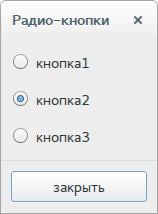
\includegraphics[width=1\linewidth]{53}}
	\caption{Радио-кнопки (RadioButtons)}
	\label{ris:image2}
\end{figure}
Файл radiobuttons.h (Для использования совместно с gtkmm 3, а не с gtkmm 2) 
\begin{lstlisting}[language=C++]
#ifndef GTKMM_EXAMPLE_RADIOBUTTONS_H
#define GTKMM_EXAMPLE_RADIOBUTTONS_H

#include <gtkmm/box.h>
#include <gtkmm/window.h>
#include <gtkmm/radiobutton.h>
#include <gtkmm/separator.h>

class RadioButtons : public Gtk::Window
{
public:
	RadioButtons();
	virtual ~RadioButtons();

protected:
	void on_button_clicked();

	Gtk::Box m_Box_Top, m_Box1, m_Box2;
	Gtk::RadioButton m_RadioButton1, m_RadioButton2, m_RadioButton3;
	Gtk::Separator m_Separator;
	Gtk::Button m_Button_Close;
};

#endif 

\end{lstlisting}
Файл radiobuttons.cpp (Для использования совместно с gtkmm 3, а не с gtkmm 2) 
\begin{lstlisting}[language=C++]
#include "radiobuttons.h"

RadioButtons::RadioButtons() :
	m_Box_Top(Gtk::ORIENTATION_VERTICAL),
	m_Box1(Gtk::ORIENTATION_VERTICAL, 10),
	m_Box2(Gtk::ORIENTATION_VERTICAL, 10),
	m_RadioButton1("button 1"),
	m_RadioButton2("button 2"),
	m_RadioButton3("button 3"),
	m_Button_Close("close")
{

	set_title("Radio-buttons");
	set_border_width(0);

	Gtk::RadioButton::Group group = m_RadioButton1.get_group();
	m_RadioButton2.set_group(group);
	m_RadioButton3.set_group(group);

	add(m_Box_Top);

	m_Box_Top.pack_start(m_Box1);
	m_Box_Top.pack_start(m_Separator);
	m_Box_Top.pack_start(m_Box2);

	m_Box2.set_border_width(10);
	m_Box1.set_border_width(10);

	m_Box1.pack_start(m_RadioButton1);
	m_Box1.pack_start(m_RadioButton2);
	m_Box1.pack_start(m_RadioButton3);

	m_RadioButton2.set_active();
	m_Box2.pack_start(m_Button_Close);

	m_Button_Close.set_can_default();
	m_Button_Close.grab_default();

	m_Button_Close.signal_clicked().connect(sigc::mem_fun(*this,
		&RadioButtons::on_button_clicked) );
	show_all_children();
}

RadioButtons::~RadioButtons()
{
}

void RadioButtons::on_button_clicked()
{
	hide(); 
}

\end{lstlisting}
Файл main.cpp (Для использования совместно с gtkmm 3, а не с gtkmm 2) 
\begin{lstlisting}[language=C++]
#include "radiobuttons.h"
#include <gtkmm/application.h>

int main(int argc, char *argv[])
{
	Glib::RefPtr<Gtk::Application> app = Gtk::Application::create(argc, argv, 		"org.gtkmm.example");

	RadioButtons buttons;

	return app->run(buttons);
}

\end{lstlisting}


